\chapter{Implementation}
\label{chap:Method}
\section{Data pre-processing}
\subsection{Dataset generation}
Nozzle simulations are carried out for 120 cases, each with a different set of Inlet 1 and Inlet 2 velocities. The velocity ratio between the two velocities lies in the range of [1,9]. Velocity ratio in our case refers to the ratio of higher velocity to that of lower velocity.
%  such that the velocity ratios between the inlets range from 1 to 9.  (Velocity ratio in our case refers to the ratio of higher velocity to that of lower velocity) 
The simulation results, i.e; the steady-state fields are logged after 1000 and 30000 time steps. The simulation results after 30000 steps are taken as the ground truth values or simply target data, whereas the input to the surrogate model are the results after 1000 steps. 
\subsection{Transformation of mesh data to graph data}
Conventional RANS solvers require substantial distances from domain boundaries to mitigate adverse effects on solutions around the region of interest. However, this is not required for the deep learning task. Hence, we narrow our attention to a small region just enclosing the nozzle as seen in Figure \ref{clipmesh}. We clip the CFD mesh appropriately and resample the velocity and pressure fields to this mesh with reduced spatial extent. We define the cell-centers on the clipped mesh and assign them as the nodes of the graph. Two adjacent cells in the mesh (cells that share an edge) corresponds to their respective nodes ($v_i$ and $v_j$) on the graph being connected by an edge $e_{ij}$. The graph connectivity is then given by the edge index data structure which comprises two lists - one stores the source node indices and the other has the destination node indices. CFD solvers typically assign pressure, velocity and other fields to each cell of the mesh whereas graphs require node features, i.e; fields defined on each node. Therefore, the cell data (fields) are converted to point data at the cell centers making it suitable for graph representation. The simulation data is then saved in a \verb|hdf5| format. This is then directly used to read $u_{x}$, $u_{y}$, $p$, $c_x$, $c_y$, and $\gamma_{\operatorname{tag}}$. The edge index data structure required for the GNN model is generated by computing adjacent cells and storing their indices in a co-ordinate list (COO) format. 
\begin{figure}[ht]
    \centering
    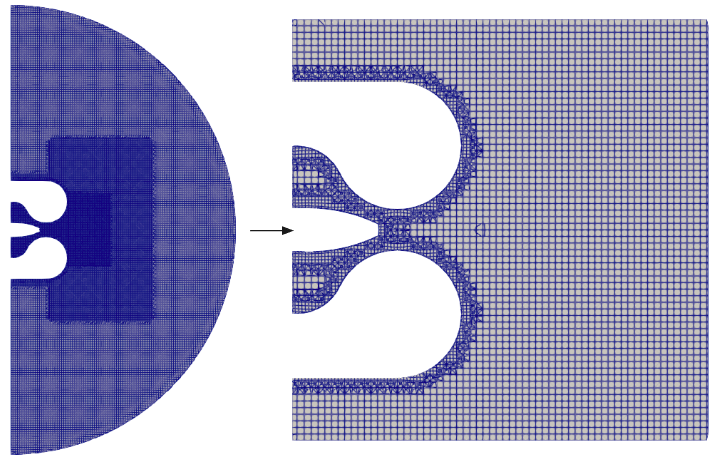
\includegraphics[width=11cm]{images/Methodology/Clipped.png}
    \caption{Region of interest}
    \label{clipmesh}
\end{figure}
\begin{figure}[ht]
    \centering
    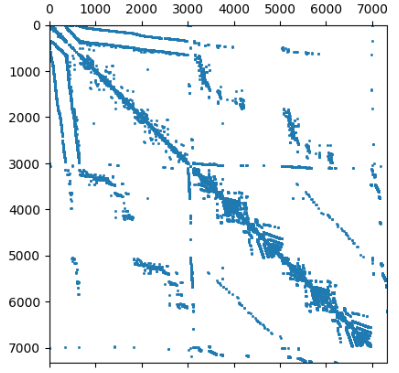
\includegraphics[width=6cm]{images/Methodology/AdjMatrix.png}
    \caption{Adjacency Matrix}
    \label{adjmat}
\end{figure}
\subsection{Model inputs and outputs}
After data pre-processing, the simulation mesh is considered as a bidirectional graph $\mathbf{G} = (\mathbf{V}, \mathbf{E})$ where the set of $N$ nodes denoted as $\mathbf{V}$ are linked by the set of edges $\mathbf{E}$ of the mesh. To construct a graph, we need,
\begin{itemize}
\item A feature description, consolidated into an $N \times D$ feature matrix $X$ (where $N$ represents the number of nodes, and $D$ denotes the number of input features).
\item The graph connectivity or relationships within nodes is represented in matrix form as an adjacency matrix, $A$ or as an edge set $E$ of the shape $2 \times P$, where $P$ is the number of pairs of connected nodes in $E$.
\end{itemize}
Let each node have $F_X$ features, and $F_Y$ predictions. The GNN maps the set of node features and edge index matrices to predictions as, 
\begin{equation}
    \mathrm{GNN}: \mathbb{R}^{{N} \times F_{\mathrm{X}}}, \mathbb{W}^{2 \times P} \rightarrow \mathbb{R}^{{N} \times F_{\mathrm{Y}}}
    \end{equation}
We then get a graph-level output $Z$ of the shape ${N} \times F_{\mathrm{Y}}$. \\
The node feature vector $\mathbf{x}_i$ and prediction vector $\mathbf{y}_i$ of interest at each node $v_i$ is given as,
\begin{equation}
    \begin{aligned}
    & \mathbf{x}_i=\left[u_{x, i}, u_{y, i},c_{x, i}, c_{y, i}, \gamma_{\operatorname{tag}, i}\right] \\
    & \mathbf{y}_i=\left[u_{x, i}, u_{y, i}, p_i\right]
    \end{aligned}
\end{equation}
where $u_{x, i}$ and $u_{y, i}$ are the node velocities in X and Y directions, $c_{x, i}$ and $c_{y, i}$ are the spatial co-ordinates of the nodes and $p_i$ is the node pressure. $\gamma_{\operatorname{tag}, i}$ is the node tag that defines which cell the node belongs to: inlet, walls or internal mesh. To summarize, our model has 5 input channels (representing node features) and 3 output channels (denoting node predictions). In addition to these channels, the GNN model also requires an edge index matrix to internally compute the adjacency matrix for the graph. 
\subsection{Data normalization}
Data normalization is performed on both input channels (node features) and output channels (target vectors), carried out in three steps outlined below.
\begin{enumerate}
\item Following common practice, we normalize all the fields of interest with respect to the magnitude of free-stream or reference velocity $u_0$ to make them dimensionless. 
\begin{equation}
    \Tilde{u}=u /\left\|u_0\right\|, \quad \Tilde{p}=p /\left\|u_0\right\|^2
\end{equation}
The latter plays a crucial role as it eliminates the quadratic scaling effect present in the pressure values of the target data, effectively flattening the solution space, thereby simplifying the task for the neural network in subsequent stages.
\item Next, we subtract the mean pressure from the dimensionless pressure values. 
\begin{equation}
\hat{p} = \Tilde{p} - p_{mean} , \quad \text{where } p_{mean} = \sum_i p_i / n
\end{equation}
$n$ is the number of training samples and $p_i$ denotes individual pressure values. Without this step, the pressure targets depict an ill-posed learning objective since the random pressure offsets in the solutions lack correlation with the inputs.
\item As a final step, every channel undergoes normalization to the range of [-1, 1] (or [0,1]). This standardization aims to mitigate errors stemming from finite numerical precision during the training period. We opt for the maximum absolute value of each quantity across the entire training dataset to normalize the data. 
\end{enumerate}
The dataset is split into 3 parts and distributed as Training Data : Validation Data : Test Data in the ratio 80:10:10. 
\section{Graph U-Net}
Here, we introduce the Graph U-Net architecture, a foundational framework for the surrogate models used in this work. We analyze the benefits and shortcomings of this model as well as explain the motivation behind developing a modified GNN.
\begin{figure}[ht]
    \centering
    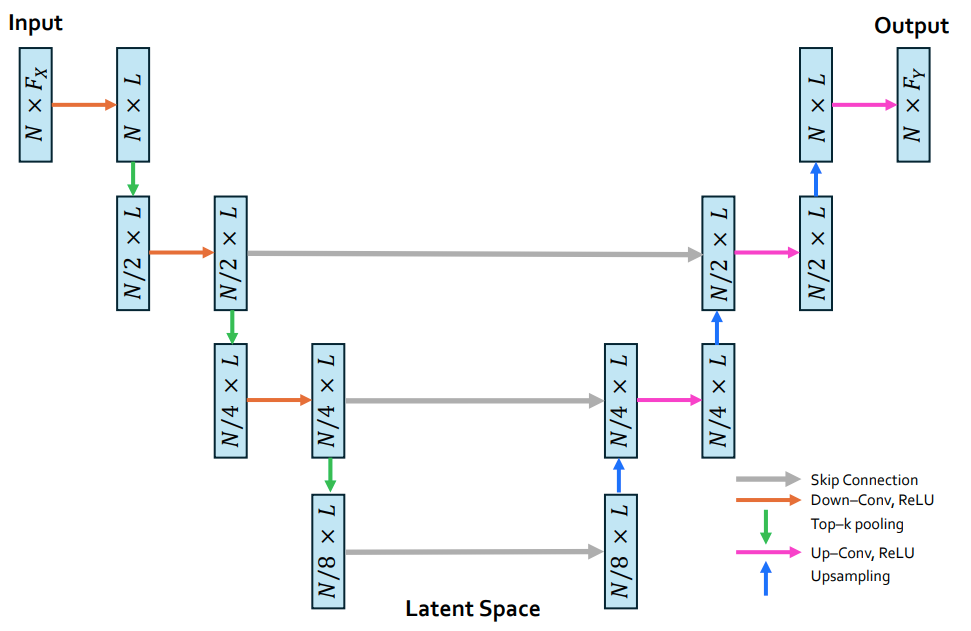
\includegraphics[width=12cm]{images/Methodology/GraphUNet.png}
    \caption{Graph U-Net architecture}
    \label{fig:GraphUnet}
\end{figure}
\subsection{GCNConv layer}
GCNs are NNs operating on graph-structured data that extend the concept of convolutional operations from regular grid-like data, such as images, to irregular and non-Euclidean graph structures, using the spectral graph convolution operation GCNConv. The GCNConv layer aggregates information from neighboring nodes and updates the representations of each node based on this aggregated information, expressed as,
\begin{equation}
h_i^{(l+1)} = \sigma \left(\sum_{j \in \mathcal{N}(i)} \frac{1}{c_{ij}} W^{(l)} h_j^{(l)} + B^{(l)} h_i^{(l)} \right)
\end{equation}
where $W^{(l)}$ and $B^{(l)}$ are the learnable weight and bias matrices for layer $l$, $\sigma$ is the activation function and $c_{ij}$ is a normalization factor. 
In contrast to filters in CNNs, the weight matrix is consistent and shared across all nodes. However, unlike pixels, nodes do not have a fixed number of neighbors. To maintain uniform value ranges across all nodes and facilitate comparability between them, we normalize the outcomes based on the degree of the nodes, i.e; the number of connections of each node. Hence, $c_{ij} = \sqrt{\text{deg(i)}}\sqrt{\text{deg(j)}}$ where, $\text{deg(i)}$ and $\text{deg(j)}$ denotes the degree of the nodes $v_i$ and $v_j$ respectively. 
% Some important aspects of graph convolutions are detailed below. 
% \begin{enumerate}
% \item \textbf{Aggregation of neighbor information:} Each node aggregates the features of its neighbors, weighted by the parameters learned in the weight matrix $W^{(l)}$. This process enables nodes to incorporate information from their local neighborhoods, capturing relational dependencies and structural patterns in the graph. 

% % The normalization factor $c_{ij}$ ensures that the aggregated features are appropriately scaled based on the connectivity of nodes.
% \item \textbf{Weight sharing:}
% The weight matrix $W^{(l)}$ is shared across all nodes, allowing the model to capture common patterns and relationships present in the graph. By sharing parameters, GCNs can effectively learn representations from limited labeled data, facilitating transfer learning and adaptation to new graphs or domains.
% \item \textbf{Hierarchical feature learning:}
% GCNConv layer enables hierarchical feature learning by iteratively aggregating information from neighboring nodes. As information propagates through multiple layers, nodes can capture increasingly abstract and high-level features of the graph. 
% \end{enumerate}
\subsection{Top-k pooling layer}
Top k-Pooling selects the $k$ nodes with the highest scores based on a specified criterion. This operation retains the most important nodes in the graph while discarding less relevant nodes, effectively downsampling the graph. It uses a pooling ratio approach, where $k \in (0, 1]$ such that the graph has $\lfloor kN \rfloor$ nodes after the pooling operation. The decision of which nodes to discard is based on a projection score computed against a learnable vector, $\mathbf{\overrightarrow{p}}$. Fully expressed, computing a pooled graph, $(X^l, A^l)$, from an input graph, $(X, A)$ can be described using the following algorithm: 
\begin{enumerate}
    \item Compute a score for each node in the graph based on node importance or feature relevance as,
    \[
\mathbf{\tilde{y}} = \frac{X \mathbf{\overrightarrow{p}}}{k||\mathbf{\overrightarrow{p}}||_2} \]
    \item Select the top $k$ nodes with the highest scores, \[ \mathbf{\overrightarrow{i}} = \text{top-k}(\mathbf{\tilde{y}}, k) \]
    \item Discard the remaining nodes and their associated edges, resulting in a downsampled graph $G^{\prime} = (V^{\prime}, E^{\prime})$ where $V^{\prime}$ contains only the selected nodes.
    \item Retain the features corresponding to the selected nodes to form the downsampled feature and adjacency matrices, \[
        X^{\prime} = (X \odot \tanh(\mathbf{\tilde{y}}))_{\mathbf{\overrightarrow{i}}}, \quad A^{\prime} = A_{\mathbf{\overrightarrow{i}},\mathbf{\overrightarrow{i}}}
       \]
\end{enumerate}
Here, $||.||_2$ represents the L2 norm, top-k selects the top-k indices, $\odot$ denotes element-wise multiplication, and $\cdot_{\mathbf{\overrightarrow{i}}}$ represents an indexing operation that extracts slices at indices specified by $\mathbf{\overrightarrow{i}}$. 
\subsection{Upsampling}
In the Graph U-Net architecture, unpooling is not a distinct operation like in traditional U-Nets. Instead, skip connections are used to implicitly perform unpooling. During decoding, downsampled features from the encoder are combined with zeros or empty features in the decoder using skip connections. This integration effectively restores spatial details and contextual information from the original input graph, ensuring that important features are retained and allowing for the recovery of detailed graph structures. Therefore, unpooling in Graph U-Net is seamlessly integrated into the skip connection mechanism, facilitating the reconstruction of the original graph resolution during decoding.
\subsection{Results and Discussions}
\subsection{Limitations of Graph U-Net}
There are several limitations to this architecture and each case is outlined below: 
\begin{enumerate}
    \item \textbf{Poor Reconstruction:} Graph U-Net lacks explicit unpooling layers, which can lead to inadequate reconstruction of the original graph structure during decoding. This omission may result in loss of detailed information and suboptimal performance in tasks requiring precise graph reconstruction.
    \item \textbf{Limited Scalability:} Originally designed for small graphs with around 100 nodes, Graph U-Net relies on dense matrix multiplications, which are memory-intensive and not scalable. This leads to memory constraints and slower training times, thus making it impractical for complex, large-scale graph data.
    \item \textbf{Computational Overhead:} Graph U-Net conducts dense adjacency matrix multiplication in the forward pass, resulting in longer training and inference times.
    \item \textbf{Limited Expressiveness:} GCNConv layers may have limited expressiveness in capturing higher-order graph structures and capturing long-range dependencies in the graph. Its optimal depth is found to be 2 or 3 layers. (CITE) Deeper models beyond 7 layers can encounter training difficulties due to increased context size per node and heightened risk of overfitting with a larger number of parameters.
\end{enumerate}
Due to these disadvantages, Graph U-Net may exhibit poor performance in terms of both accuracy and efficiency, particularly for complex geometries or large-scale datasets. Hence, there is a paramount necessity to rely on a modified GNN architectures for our work.
\section{Proposed architecture}
In this section, we discuss the architecture of the proposed GNN surrogate model in detail. We elucidate the novel components in the architecture and the adjustments made on the original Graph U-Net framework. Then, we go on to provide comprehensive details on the hyperparameters and other implementation specifics of the proposed GNN model. Finally, we demonstrate the training process and share the predictions, training and test results obtained for the CFD application. The GNN is developed on the Pytorch deep learning framework using the Pytorch Geometric (PyG) library. Training and testing are performed on V100 GPU compute node using a single GPU (nVidia Tesla V100).\\
There are 4 different surrogate models proposed, each with a slight variation of the Graph U-Net architecture which is considered as the baseline model and referred to as \textit{BL}. They are, 
\begin{enumerate}
    \item \textit{BL + knn:} This model uses the k-NN interpolation technique used in PointNet++ \cite{pnpp} for unpooling or upsampling of features instead of relying on skip connections. The downsampled features at different depths (levels of coarsening) are stored so that the upsampled node co-ordinates required for k-NN interpolation can be obtained from $[c_{x}, c_{y}]$ at the downsampled feature of the same depth.
    \item \textit{BL + SAGE + knn:} In this surrogate, we replace the GCNConv layers of \textit{BL + knn} with GraphSAGE. 
    \item \textit{BL + crsn + knn:} In this surrogate, we first obtain the set of coarsened meshes through incremental decimation of the CFD mesh by running a Python script on Paraview. With the mesh indices and co-ordinates of the low-resolution mesh nodes, we compute the downsampled features for the graph using the sampling operator described in the subsection \ref{SO}. Thus, we implement the pooling operation with the help of sampling operator and perform unpooling operation using k-NN interpolation. 
    \item \textit{BL + SAGE + crsn + knn:} Similar to the previous model in every detail, the only difference in this model is that it uses GraphSAGE layers instead of the GCNConv layers as convolutions.
    % \item \textit{BL + MoNet + sampl. + knn:} This model is also similar to \textit{BL + crsn + knn}, but it applies MoNet blocks for up convolutions and down convolutions. 
\end{enumerate}
% \subsection{Multi-Resolution Graph Net Architecture}
\section{Model hyperparameters and training parameters}

\subsection{Parameter study of graph layers}
The design choices in the model architecture can impact the overall performance of the model. 
